% \begin{figure}
%     \centering
%     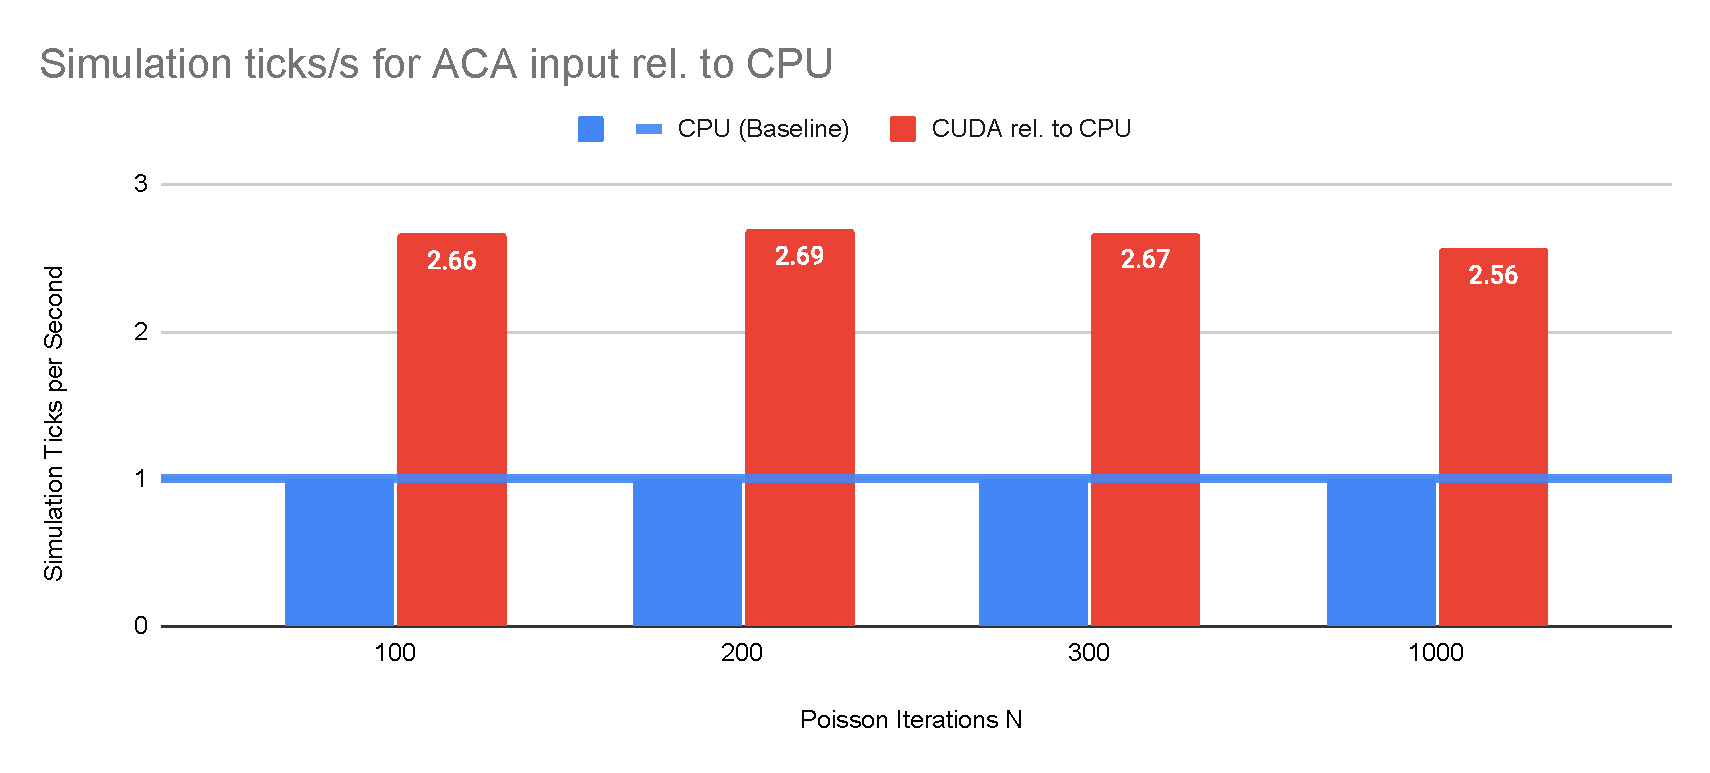
\includegraphics[width=\linewidth]{Ch62Results/figures/temp_ticks_per_second_vs_iters_rel_cpu_aca.pdf}
%     \caption{Simulation Tick Speed relative to CPU}
%     \label{fig:results:ticks_per_second_bar_rel_cpu_aca}
% \end{figure}

\begin{figure}
    \centering
    \resizebox{\linewidth}{!}{%
    \begin{tikzpicture}
    \begin{axis}[
        % title={Simulation Tick Speed},
        ylabel={Tick Rate (\si{\per\second})},
        xlabel={Poisson Iterations N},
        % xtick = {100, 200, 300, 400},
        xtick=data,
        symbolic x coords={100, 200, 300, 1000},
        width=\linewidth,
        height=20em,
        bar width=30pt,
        x tick style = transparent,
        ybar,
        enlarge x limits=0.25,
        ymin=0, ymax=3
    ]
    
    \addplot[ fill=blue] table [x=iters, y=cpu_speed_rel, col sep=semicolon, ignore chars={\,}] {Ch62Results/figures/data/ticks_per_second.csv};
    \addlegendentry{CPU};
    
    \addplot[ fill=red] table [x=iters, y=cuda_speed_rel, col sep=semicolon, ignore chars={\,}] {Ch62Results/figures/data/ticks_per_second.csv};
    \addlegendentry{CUDA};

    
    \draw [black, style={line width=2pt}] ({rel axis cs:0,0}|-{axis cs:100,1.0}) -- ({rel axis cs:1,0}|-{axis cs:100,1.0});% node [pos=0.33, above] {KPI};
    
    \end{axis}
    \end{tikzpicture}
    }
    
    \caption{Simulation Tick Speed relative to CPU}
    \label{fig:results:ticks_per_second_bar_rel_cpu_aca}
\end{figure}